%%--------------------------------Packages and stuff--------------------------------%%
\documentclass[11pt]{article}
\usepackage[utf8]{inputenc} %input type
\usepackage{siunitx}
\usepackage{lipsum} %for nonsense text
\usepackage{verbatim} %for multiline comments
\usepackage{fancyhdr} %header&footer
\usepackage{natbib} %bibliography
\usepackage{hyperref} %hyperlinks
\hypersetup{
     colorlinks   = true,
     citecolor    = black,
     urlcolor = black,
     linkcolor = black
}
\usepackage[nottoc,notlot,notlof]{tocbibind} %for showing  bibliography in toc
\usepackage{listings}
\usepackage{textcomp}
\usepackage{mathtools}
\usepackage{enumitem}
\setitemize{noitemsep,topsep=0pt,parsep=0pt,partopsep=0pt}
\renewcommand\labelitemi{\scriptsize$\bullet$}
\usepackage{array}
\newcolumntype{N}{@{}m{0pt}@{}}
\usepackage{indentfirst} %indent first paragraph
\setlength{\parindent}{4mm}

%%--------------------------------Figures setup--------------------------------%%
\usepackage{graphicx} %for  images
\usepackage{grffile} %for pngs
\graphicspath{ {images/} } %images path
%%--------------------------------End of figures setup--------------------------------%%

%%--------------------------------Geometry aka page layout setup--------------------------------%%
\usepackage{geometry} %geometry aka page layout
\geometry{
  a4paper,
  left=25mm,
  right=25mm,
  top=25mm,
  bottom=25mm,
  head=25mm
}
%%--------------------------------End of geometry aka page layout setup--------------------------------%%

\usepackage{fontspec}
\usepackage{minted}

%%--------------------------------Caption setup--------------------------------%%
\usepackage{caption}
\DeclareCaptionStyle{mystyle}
  {format=plain,
    textformat=period,
    justification=RaggedRight,
    singlelinecheck=true,
  }% all captions are left aligned

\DeclareCaptionStyle{singlelinecentered}
  [justification=Centering]% centered if single line and no `singlelinecheck=false`
  {style=mystyle}% other captions are left aligned
  
\captionsetup{style=singlelinecentered}
%%--------------------------------End of caption setup--------------------------------%%

%%--------------------------------Title formatting--------------------------------%%
\usepackage{titlesec}
%%-----Spacing-----%%
\titleformat{\section}[hang]{}{\thesection}{0.4em}{}
\titleformat{\subsection}[hang]{}{\thesubsection}{0.4em}{}
\titleformat{\subsubsection}[hang]{}{\thesubsubsection}{0.4em}{}
\titleformat{\paragraph}[hang]{}{\theparagraph}{0.4em}{}
\titlespacing{\section}{0mm}{5mm}{2mm}
\titlespacing{\subsection}{0mm}{5mm}{2mm}
\titlespacing{\subsubsection}{0mm}{5mm}{2mm}
\titlespacing{\paragraph}{0mm}{5mm}{2mm}

%%-----Font-----%%
\titleformat*{\section}{\Large\bfseries\sffamily}
\titleformat*{\subsection}{\large\bfseries\sffamily}
\titleformat*{\subsubsection}{\normalsize\bfseries\sffamily}
\titleformat*{\paragraph}{\normalsize\bfseries\sffamily}
%%--------------------------------End of Title formatting--------------------------------%%

%%--------------------------------ToC setup--------------------------------%%
\usepackage{tocloft}
\setcounter{secnumdepth}{5}
\setcounter{tocdepth}{5}
\renewcommand\cftsecleader{\cftdotfill{\cftdotsep}}
\setlength{\cftfigindent}{0pt}
\setlength{\cfttabindent}{0pt}
%\newcommand{\cfttocnumwidth}{}
\renewcommand{\listfigurename}{\sffamily{\Large{Kazalo slik}}}
\renewcommand{\listtablename}{\sffamily{\Large{Kazalo tabel}}}
\renewcommand{\contentsname}{Kazalo}
\renewcommand{\cfttoctitlefont}{\Large\bfseries\sffamily}
%\setlength{\cfttocnumwidth}{1mm}
%%--------------------------------End of ToC setup--------------------------------%%
%%--------------------------------Acronyms and glossaries setup--------------------------------%%
\usepackage[acronym, toc]{glossaries}
\makeglossaries
%%--------------------------------Acronyms--------------------------------%%
\newglossaryentry{ssh}{type=\acronymtype, name={SSH}, description={Secure Shell}, first={Secure Shell (SSH)\glsadd{sshg}}, see=[Glossary:]{sshg}}
%%--------------------------------End of Acronyms--------------------------------%%

%%--------------------------------Glossary--------------------------------%%
\newglossaryentry{guig}{name={GUI},
    description={``The graphical user interface, is a type of user interface that allows users to interact with electronic devices through graphical icons and visual indicators."\cite{wikiGUI}}}
%%--------------------------------End of Glossary--------------------------------%%
%%--------------------------------End of acronyms and glossaries setup--------------------------------%%

%%--------------------------------Custom commands--------------------------------%%
\newcommand{\shellcmd}[1]{\\\indent\indent\texttt{\normalsize\$ #1}\\}
\newcommand{\shellcmdn}[1]{\\\texttt{\normalsize\$ #1}\\}
\newcommand{\source}[2]{\caption{#1}\vspace{-1.5mm}{\tiny{\url{{#2}}}} }
\newcommand{\numpara}[1]{\paragraph{{#1}}\mbox{}\vspace{0mm}}
%%--------------------------------End of Custom commands--------------------------------%%

%%--------------------------------End of packages and stuff--------------------------------%%

%%--------------------------------Beginning of the document--------------------------------%%
\begin{document}

\renewcommand{\theFancyVerbLine}{
  \sffamily\textcolor[rgb]{0.5,0.5,0.5}{\scriptsize\arabic{FancyVerbLine}}}
%%--------------------------------Beginning of the title page--------------------------------%%
\begin{titlepage}
\thispagestyle{empty}
   \center
   \fancyhead{}
   \large{Šolski center Celje, Srednja šola za kemijo, elektrotehniko in računalništvo}\\[1.5cm]
   \vspace*{\fill}
   \begin{center}
   \Huge{\bfseries Pametna garažna vrata}\\
   \vspace{1mm}
   \large{Raziskovalna naloga}
   \end{center}
   \vspace*{\fill}
   	%------------------------------------------------
	%	Author(s)
	%------------------------------------------------
	
	\begin{minipage}{0.4\textwidth}
		\begin{flushleft}
		\vspace{4.5mm}
			\large
			\texttt{Avtor}\\
			Boštjan \textsc{Planko}, R-4.A \\ %Author's name
			%\vspace{0.2cm}
			%\texttt{Submission date} \\
			%\large{December 7, 2017}
		\end{flushleft}
	\end{minipage}
	~
	%------------------------------------------------
	%	Supervisor(s)
	%------------------------------------------------
	\begin{minipage}{0.5\textwidth}
		\begin{flushright}
			\large
			\texttt{Mentor}\\
			Borut \textsc{Slemenšek} % Supervisor's name
		\end{flushright}
	\end{minipage}
	~
	%------------------------------------------------
	%	Date
	%------------------------------------------------
	\begin{minipage}{0.5\textwidth}
		\begin{center}
		    \vspace{3mm}
			\large{Celje, \today}
		\end{center}
	\end{minipage}
	\fancyfoot{}
\end{titlepage}
%%--------------------------------End of title page--------------------------------%%

%%--------------------------------Beginning of abstract--------------------------------%%
\newpage
\thispagestyle{empty}
\section*{Povzetek}

\section*{Ključne besede}
%%--------------------------------End of abstract--------------------------------%%

%%--------------------------------Beginning of ToC--------------------------------%%
\renewcommand{\baselinestretch}{0.90}\normalsize
\newpage
\pagenumbering{gobble}
\thispagestyle{empty}
\tableofcontents
\listoftables
\listoffigures
\renewcommand{\baselinestretch}{1.0}\normalsize
%%--------------------------------End of ToC--------------------------------%%
\newpage

%%--------------------------------Beginning of head & foot--------------------------------%%
\pagestyle{fancy}
\fancyhead{}
\fancyhead[C]{Pametna garažna vrata}
\fancyfoot{}
\fancyfoot[C]{\thepage}
%%--------------------------------End of head & foot--------------------------------%%

%%--------------------------------Beginning of Section 1 aka Intro--------------------------------%%
\pagenumbering{arabic}
\setcounter{page}{4}
\section{Uvod}
\subsection{Opis problema}
Problem današnjih garažnih vrat je, da jih je običajni možno odpreti samo na dva načina. S priloženim daljincem ali s tipko, običajno nameščeno na notranji strani garažnih vrat. Če želimo torej garažna vrata odpretni moramo bitjt ali v garaži ali pa moramo imeti pri sebi daljinec. To pa je v vsakdanjem življenju nepraktično, sploh v primeru, ko pri hiši živi veliko ljudi, vsi pa rabijo dostop do garaže.

V tej nalogi bom predstavil svojo idejo, pametna garažna vrata, kot sem si jih zamislil in poskušal realizirati.

\subsection{Cilji}
Za raziskovalno nalogo, sem si postavil naslednje cilje:
\begin{itemize}
    \item Garažna vrata bo možno upravljati preko telefona
    \item Garažna vrata bo možno upravljati preko spletne strani
    \item Raspberry Pi bo spremljal ali je avto v garaži ali ne in glede na to samodejno zapiral garažna vrata
    \item Raspberry Pi bo spremljal temperaturo v garaži in jih samodejno zaprl v primeru prenizke ali previsoke temperature
    \item Raspberry Pi bo samodejno zaprl garažna vrata, če ostanejo odprta po določeni uri
    \item Raspberry Pi nas bo preko potisnih obvestil obveščal o spremembi stanja garažnih vrat
    \item Raspberry Pi bo beležil kdo in kdaj je aktiviral garažna vrata
    \item uporabnik bo imel možnost preklicati samodejno zapiranje vrat
\end{itemize}
 
 \newpage
\section{Izbira komponent}
  Ker ne potrebujem veliko precesorske moči, hkrati pa želim, da je moj projekt kar se da kompakten kot krmilnik izberem Raspberry Pi Zero W. To je najmanjša verzija Raspberry Pi-ja, z že vgrajenim WiFi-jem in Bluetoothom. Slednja bosta pri projektu najverjetneje potrebna.
  
  Za upravljanje garažnih vrat bom uporabil 1-kanalni rele. Le tega bom sprogramiral tako, da se bo obnašal kot tipka tj. zaprl se bo za kratek časovni interval prib. 0.5s, nato pa se znova odprl. Nameščen bo v bližini že obstoječe tipke, ki se uporablja za upravljanje garažnih vrat. Z le to bo vzporedno vezan.
  
  Za spremljanje stanja garažnih vrat bom uporabil reed stikala. In sicer dve stikali ter in magnet. Stikali bosta nameščeni na ogrodje vrat, medtem ko bo magnet nameščen neposredno na garažna vrata.
  
  Za spremljanje temperature v garaži uporabim 1-Wire digitalni element.... (nevem imena zle). Le ta bo nameščen nekje v garaži, po možnosti meter od tal, na najmanj prepišnem mestu v garaži.
  
  Ultrazvočni senzor, s katerim bom preverjal ali je avto v garaži ali ne, bo nameščen ali na stropbu garaže, najverjetneje pa kar na motorju garažnih vrat.
  
  Ker želim, da bo mogoče v garaži preveriti ternutno temperaturo ter čas, bom uporabil tudi 16x2 LCD zaslon.
  
  Poleg že naštetih komponent bo uporabil še dve LED diodi in dve tipki. Le te bodo paroma uporabljene kot indikator stanja avta oziroma temperature v garaži. Če bo naprimer garaža odprta in bo vanjo pripeljal avto, se bo pognal program, ki bo po določenem času samodejno zaprl vrata. Istočasno, bo začela utripati ustrezna LED dioda, uporabnik pa bo imel s pritiskom tipke možnost da prekliče samodejno zapiranje garaže. Pri temperaturi je namen LED diode in tipke enak, le da spremljamo temperaturo v garaži.
\section{Priprava Raspberry Pi-ja}
 Da bom lahko uporabljal Raspberry Pi, moram najprej naložiti usterzen opreacijski sistem na Raspberry Pi. Ker za svoj projekt ne potrebujem grafičnega vmesnika, na Raspberry Pi namestim Raspbian Lite. To storim tako, da iz [uradne strani](https://www.raspberrypi.org/downloads/raspbian/) Raspberry Pi prenesem Raspbian Stretch Lite. Nato sledim [navodilom](https://www.raspberrypi.org/documentation/installation/installing-images/README.md) za namestitev operacijskega sistema na microSd kartico, ki jo nato vstavim v Raspberry Pi.
 
Ker do Raspberry Pi-ja že od samega začetka nimam dostopa preko tipkovnice, moram pred zagonom omogočiti še SSH ter vnesti podatke, ki jih Raspberry Pi potrebuje za povezavo na WiFi dostopno točko. Da omogočim SSH, na boot particijo microSD katrice dodam datoteko ssh. Da pa se bo Raspberry Pi lahko povezal na WiFi dostopno točko, moram na boot particiji ustvariti datoteko wpa\_supplicant.conf, v katero vnesem naslednje:

\begin{minted}[mathescape,
               linenos,
               numbersep=5pt,
               gobble=0,
               frame=lines,
               framesep=2mm]{bash}
  
country=SI
ctrl_interface=DIR=/var/run/wpa_supplicant GROUP=netdev
update_config=1
network={
	ssid="imeDostopneTpočke"
	psk="geslo"
	key_mgmt=WPA-PSK
}
\end{minted}

Nato microSD kartico vstavim v Raspberry Pi in priključim napajanje.
\\

Nato se iz terminala na svojem računalniku preko SSH povežem na Raspberry Pi:

\begin{minted}[mathescape,
               linenos,
               numbersep=5pt,
               gobble=0,
               frame=lines,
               framesep=2mm]{python}
  
ssh pi@IP_RaspberryPi #uporabnik pi, privzeto geslo pa je raspberry
\end{minted}

Ko je povezava vzpostavljena uporabim ukaz \textit{passwd pi}, da spremenim geslo uporabnika pi.

Nato zaženem ukaz \textit{sudo raspi-config}
\begin{figure}[h]
\centering
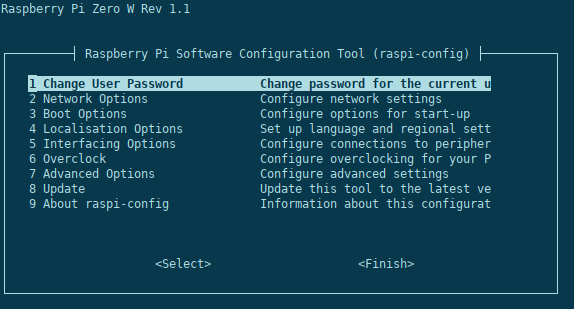
\includegraphics[width=10cm, height=5cm]{images/raspi-config.png}
\caption{raspi-config: Glavni meni}
\end{figure}

Pojavi se meni po katerem se premikam s pomočjo tipkovnice.

Tukaj nastavim vse potrebno:
\begin{itemize}
    \item hostname spremenim iz "raspberrypi" v "projectPi"
    \item časovno območje nastavim na Europe/Ljubljana
    \item omogočim SPI, I2C in 1-Wire (vse to bom potreboval za priklop senzorjev)
    \item razširim datotečni sistem
\end{itemize}

Preden namestim kakršnekoli nove pakete, je potrebno sistem posodobiti:

\begin{minted}[mathescape,
               linenos,
               numbersep=5pt,
               gobble=0,
               frame=lines,
               framesep=2mm]{python}
  
sudo apt update && sudo apt upgrade -y
\end{minted}

Ker bom program za upravljanje garažnih vrat napisal v Pythonu, le tega namestim na Raspberry Pi:
\begin{minted}[mathescape,
               linenos,
               numbersep=5pt,
               gobble=0,
               frame=lines,
               framesep=2mm]{python}
  
sudo apt install python python-pip
\end{minted}

Ker pa bom uporabil tudi LCD, moram namestiti še RPILCD knjižnico:

\begin{minted}[mathescape,
               linenos,
               numbersep=5pt,
               gobble=0,
               frame=lines,
               framesep=2mm]{python}
  
sudo pip install RPLCD
\end{minted}

S tem je priprava Raspberry Pi-ja zaključena.

\section{Priključitev komponent}
\subsection{Rele}
Sam priklop releja je zelo enostaven. Modul z relejem ima tri priključke: VCC, GND in IN1. VCC priključek povežem na 5V pin. GND priključim na GND pin. Za IN1 izberem BMC pin 16.

\subsection{Reed stikali}
Priključitev reed stikal je v osnovi zelo enostavna. Paziti je treba, da imamo NO (Normally Open) in ne NC (Normally Closed) stikala. Nato en del stikala povežemo na 3.3V, drugi del pa na enega izmed GPIO pinov. Zaj sem za eno stikalo (garaža odprta) priklopil na BCM pin 5, drugega (garaža zaprta) pa na BCM pin 6.

Po priklopu, je treba paziti, da v programu ne pozabimo nastaviti pull-down uporov, oba pina pa morata biti nastavljena kot vhodna. Tako ima pin vrednost 1, če je stikalo zaprto in vrednost 0, če je stikalo odprto.

\subsection{Ultrazvočni senzor razdalje HC-SR04}
Ker je bilo to prvič, da sem uporabljal ultrazvočni senzor razdalje na Raspberry Pi, sem si pomagal z vodičem na ModMyPi\cite{ModMyPi_us}.

Senzor ima štiri pine: VCC, GND, Trig, Echo. VCC povežem na 5V. GND, povežem na GND pin, Trig na BCM pin 11, Echo pa najprej preko \SI{1}{\kohm} upora na BCM pin 20, nato pa še preko \SI{2}{\kohm} na GND.

Da pridobim razdaljo, uporabim naslednjo metodo:
\begin{minted}[mathescape,
               linenos,
               numbersep=5pt,
               gobble=0,
               frame=lines,
               framesep=2mm]{python}
def checkCar():  
    GPIO.output(GPIO_VARS_DICT['TRIG'], False)
    time.sleep(0.001)

    GPIO.output(GPIO_VARS_DICT['TRIG'], True)
    time.sleep(0.00001)
    GPIO.output(GPIO_VARS_DICT['TRIG'], False)

    while GPIO.input(GPIO_VARS_DICT['ECHO'])==0:
      pulse_start = time.time()

    while GPIO.input(GPIO_VARS_DICT['ECHO'])==1:
      pulse_end = time.time()

    pulse_duration = pulse_end - pulse_start
    distance = pulse_duration * 17150

    return round(distance, 2)
\end{minted}

\subsection{DS18B20 temperaturni senzor}
Ker je bilo to prvič, da sem v projektu uporabil DS18B20 senzor temperature, sem si pomagal z vodičem na PiMyLifeUp\cite{PiMyLifeUp_DS18B20}.

Sam priklop je povsem enostaven. Vse kar potrebujemo je DS18B20 senzor temperature in pa 4.7\SI{4.7}{\kohm} upor. Vcc nogico senzorja povežem na 3.3V. GND nogico na GND. DATA nogico pa na BCM pin 19. Upor namestim med 3.3V in DATA nogico senzorja.
\begin{figure}[h]
\centering
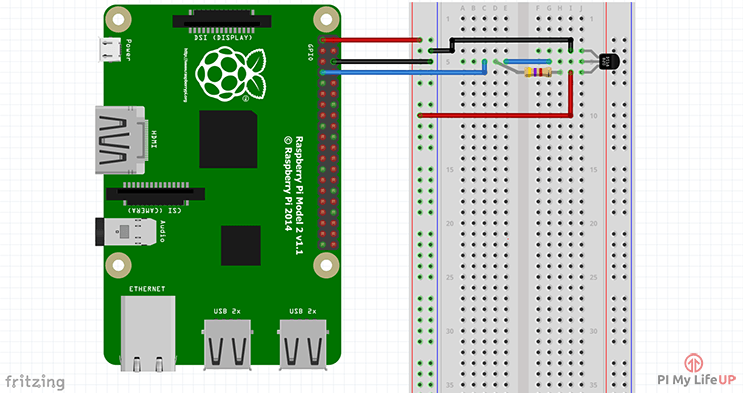
\includegraphics[width=0.5\textwidth]{images/DS18B20_diagram.png}
\caption{Priklop DS18B20}
\end{figure}
\newpage
\subsection{LCD zaslon}
Tudi priklop LCD zaslona je bil zame nekaj novega. Zato sem si pomagal z vodičem na circuitbasics.com\cite{CB_LCD}.
Za priklop potrebujem:
\begin{itemize}
    \item LCD zaslon
    \item 2 \SI{10}{\kohm} potenciometra
\end{itemize}
LCD zaslon priklopim na Raspberry Pi kot je prikazano na spodnji sliki.
\begin{figure}[h]
\centering
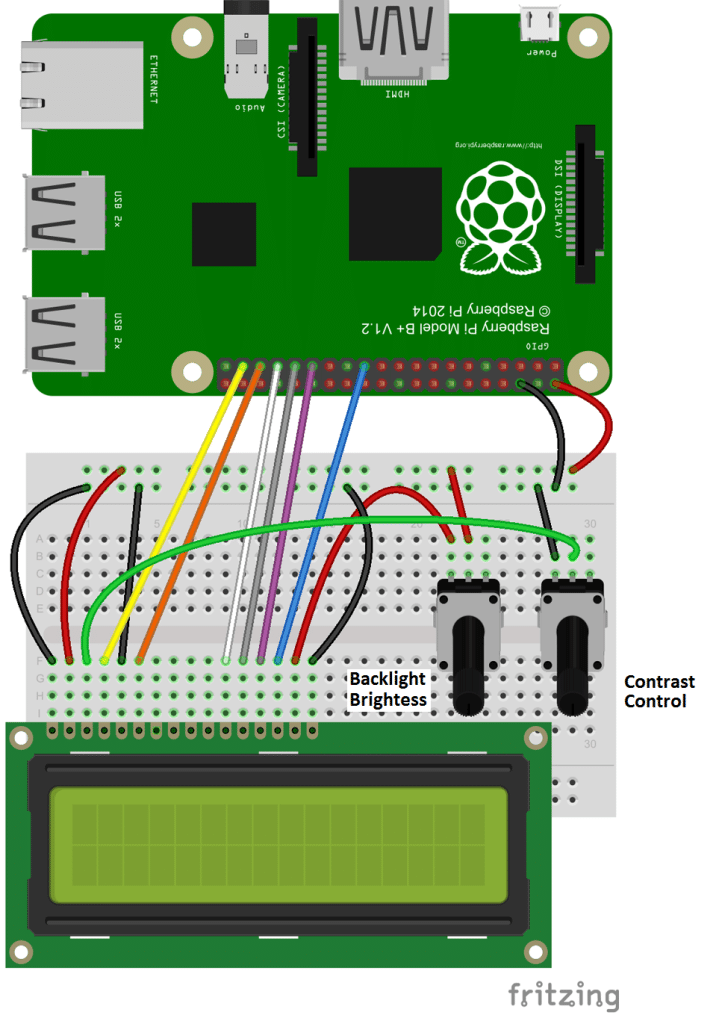
\includegraphics[width=0.5\textwidth]{images/LCD_4bit.png}
\caption{Priklop LCD zaslona}
\end{figure}
\newpage
\subsection{Tipki in LED diodi}
Priklop tipk in LED diod je zelo enostaven. Tipki povežem preko 3.3V na poljuben GPIO pin, pri tem pazim le, da je pin nastavljen kot vhodni in da je omogočen notranji pull down upor.
LED diodi pa priklopim preko \SI{270}{\ohm} uporov iz poljubnega GPIO pina na GND. GPIO pin mora biti nastavljen kot izhodni.
\section{Programske rešitve}
\subsection{Premikanje garažnih vrat}
\begin{minted}[mathescape,
               linenos,
               numbersep=5pt,
               gobble=0,
               frame=lines,
               framesep=2mm]{python}
  
def toggleGarage():
    GPIO.output(GPIO_VARS_DICT['RELAY'], 0)
    time.sleep(.5)
    GPIO.output(GPIO_VARS_DICT['RELAY'], 1)
\end{minted}
\subsection{Preveranje stanja garažnih vrat}

\subsection{Spremljanje temperature}

\subsubsection{Izpisovanje temperature na LCD}


\subsubsection{Samodejno zapiranje ob neprimerni temperaturi}


\subsection{Samodejno zapiranje glede na avto}


\subsection{Če garažnih vrat ni možno zapreti}
\begin{minted}[mathescape,
               linenos,
               numbersep=5pt,
               gobble=0,
               frame=lines,
               breaklines=true,
               framesep=2mm]{python}
  
def doorAjar():
    for attempts in range(0, TIMEOUTS_VARS_DICT['AJAR_CLOSE_ATTEMPTS']):
        toggleGarage()
        for x in range(0, TIMEOUTS_VARS_DICT['AJAR_TIMEOUT']):
            if checkDoor() != 'priprta':
                break
            time.sleep(1)
        if checkDoor() == 'zaprta':
            break
        elif checkDoor() == 'odprta':
            closeDoor()
\end{minted}

\subsection{Konfiguracijska datoteka}
\subsubsection{Datoteka}
\begin{minted}[mathescape,
               linenos,
               numbersep=5pt,
               gobble=0,
               frame=lines,
               breaklines=true,
               framesep=2mm]{python}
  
[gpio]
TRIG = 11
ECHO = 20
RELAY = 16
OVERRIDE_CAR = 26
OVERRIDE_TEMP = 12
LED_MONITOR_CAR = 13
LED_MONITOR_TEMP = 21
REED_OPEN = 5
REED_CLOSED = 6
\end{minted}
\subsubsection{Branje iz datoteke}
\begin{minted}[mathescape,
               linenos,
               numbersep=5pt,
               gobble=0,
               frame=lines,
               breaklines=true,
               framesep=2mm]{python}
  
def readConf(section, vars, val_dict):
    configParser = ConfigParser.RawConfigParser(allow_no_value=True)
    configParser.read(os.environ['HOME']+'/.garage/garage.conf')
    for value in vars:
        val_dict[value] = int(configParser.get(section, value))
\end{minted}
%%--------------------------------End of Section 1 aka Intro--------------------------------%%
\newpage
\section{Zaključek}
%%--------------------------------Beginning of Acronyms & Glossary--------------------------------%%
\newpage
\clearpage
 
\printglossary[type=\acronymtype]
 
\printglossary[type=main]
%%--------------------------------End of Acronyms & Glossary--------------------------------%%

\newpage

%%--------------------------------Beginning of Bibliography--------------------------------%%
\begin{flushleft}

\bibliographystyle{plain}
\bibliography{sources.bib}
\end{flushleft}
%%--------------------------------End of Bibliography--------------------------------%%

\end{document}
%%--------------------------------End of document--------------------------------%%
